\documentclass{article}
\usepackage[left=4cm, right=4cm, top=3cm, bottom=3cm]{geometry}
\usepackage{amsmath}
\usepackage{hyperref}
\DeclareMathOperator*{\argmax}{\arg\!\max}
\usepackage{amssymb}
\usepackage[utf8]{inputenc}
\usepackage{graphicx}
\graphicspath{{../images/}}
\usepackage{csquotes}
\setlength{\parindent}{0cm}
\usepackage[font={small, it}]{caption}

\newcommand\RepoAddress{https://github.com/enjeeneer/sutton_and_barto}
\newcommand\ProgrammingExercise{This is a programming exercise, the relevent code can be found on \href{\RepoAddress}{my GitHub}.}

\title{Reinforcement Learning: An Introduction - Notes}
\author{Scott Jeen}
\date{\today}

\begin{document}
	
\maketitle
\tableofcontents
\section{Introduction }	
\subsection{Overview}
\begin{itemize}
	\item Supervised learning = learning with labels defined by human; Unsupervised learning = finding patterns in data. Reinforcement learning is a 3rd machine learning paradigm, in which the agent tries to maximise its reward signal.
	\item Exploration versus exploitation problem - agent wants to do what it has already done to maximise reward by exploitation, but there may be a bigger reward available if it were to explore.
	\item RL is based on the model of human learning, similar to that of the brain's reward system.
\end{itemize}

\subsection{Elements of Reinforcement Learning}
\begin{description}
	\item[Policy] Defines the agent's way of behaving at any given time. It is a mapping from the perceived states of the environment to actions to be taken when in those states.
	\item[Reward Signal] The reward defines the goal of the reinforcement learning problem. At each time step, the environment sends the RL agent a single number, a \textit{reward}. It is the agent's sole objective to maximise this reward. In a biological system, we might think of rewards as analogous to pain and pleasure. The reward sent at any time depends on the agent's current action and the agent's current state. If my state is hungry and I choose the action of eating, I receive positive reward.
	\item[Value function] Reward functions indicate what is good immediately, but value functions specify what is good in the long run. The value function is the total expected reward an agent is likely to accumulate in the future, starting from a given state. E.g. a state might always yield a low immediate reward, but is normally followed by a string of states that yield high reward. Or the reverse. Rewards are, in a sense, primary, whereas values, as predictions of rewards, are secondary. Without rewards there could be no value. Nevertheless, it is values with which we are most concerned when evaluating decisions. We seek actions that bring the highest value, not the highest reward, because they obtain the greatest amount of reward over the long run. Estimating values is not trivial, and efficiently and accurately estimating them is the core of RL.
	\item[Model of environment (optionally)] Something that mimics the behaviour of the true environment, to allow inferences to be made about how the environment will behave. Given a state and action, the model might predict the resultant next state and next reward. They are used for \textit{planning}, that is, deciding on a course of action by considering possible future situations before they are actually experienced. 
\end{description}

	
	
	
	

\section{Multi-arm Bandits}

RL evaluates the actions taken rather than instructs correct actions like other forms of learning.

\subsection{An n-Armed Bandit Problem}
\textbf{The problem}
\begin{itemize}
\item You are faced repeatedly with a choice of \textit{n} actions.
\item After each choice, you receive a reward from a stationary probability distribution.
\item Objective is to maximise total reward over some time period, say 100 time steps.
\item Named after of slot machine (one-armed bandit problem), but \textit{n} levers instead of 1.
\item Each action has an expected or mean reward based on its probability distribution. We shall call thjs the \textit{value} of the action. We do not know these values with certainty.
\item Because of this uncertainty, there is always an exploration vs exploitation problem. We always have one action that we deem to be most valuable at any instant, but it is highly likely, at least initially, that there are actions we are yet to explore that are more valuable.
\end{itemize}

\subsection{Action-Value Methods}
The estimated action value is
\begin{equation} \label{eq: estimated value}
	Q_t(a) = \frac{R_1+R_2+\cdots+R_{N_t(a)}}{N_t(a)}
\end{equation}

The true value (mean reward) of an action is \(q\), but the estimated value at the \textit{t}th time-step is Q(a), given by Equation \ref{eq: estimated value} (our estimate after \textit{N} selections of an action yielding \textit{N} rewards).\\

The greedy action selection method is
\begin{equation} \label{eq: argmax}
A_t =\argmax_a Q_t(a)
\end{equation}

\begin{itemize}
	\item Simplest action selection rule is to select the action with the highest estimated value.
	\item $\argmax_a$ means the value of \(a\) for which \(Q_t\) is maximised.
	\item \(\epsilon\)-greedy methods are where the agent selects the greedy option most of the time, and selects a random action with probability \(\epsilon\).
	\item Three algorithms are tried: one with \(e\)=0 (pure greedy), one with \(e\)=0.01 and another with \(e\)=0.1
	\item Greedy method gets stuck performing sub-optimal actions.
	\item \(e\)=0.1 explores more and usually finds the optimal action earlier, but never selects it more that 91\% of the time.
	\item \(e\)=0.01 method improves more slowly, but eventually performs better than the e=0.1 method on both performance measures.
	\item It is possible to reduce \(e\) over time to try to get the best of both high and low values.
\end{itemize}
\begin{figure}
	\centering
	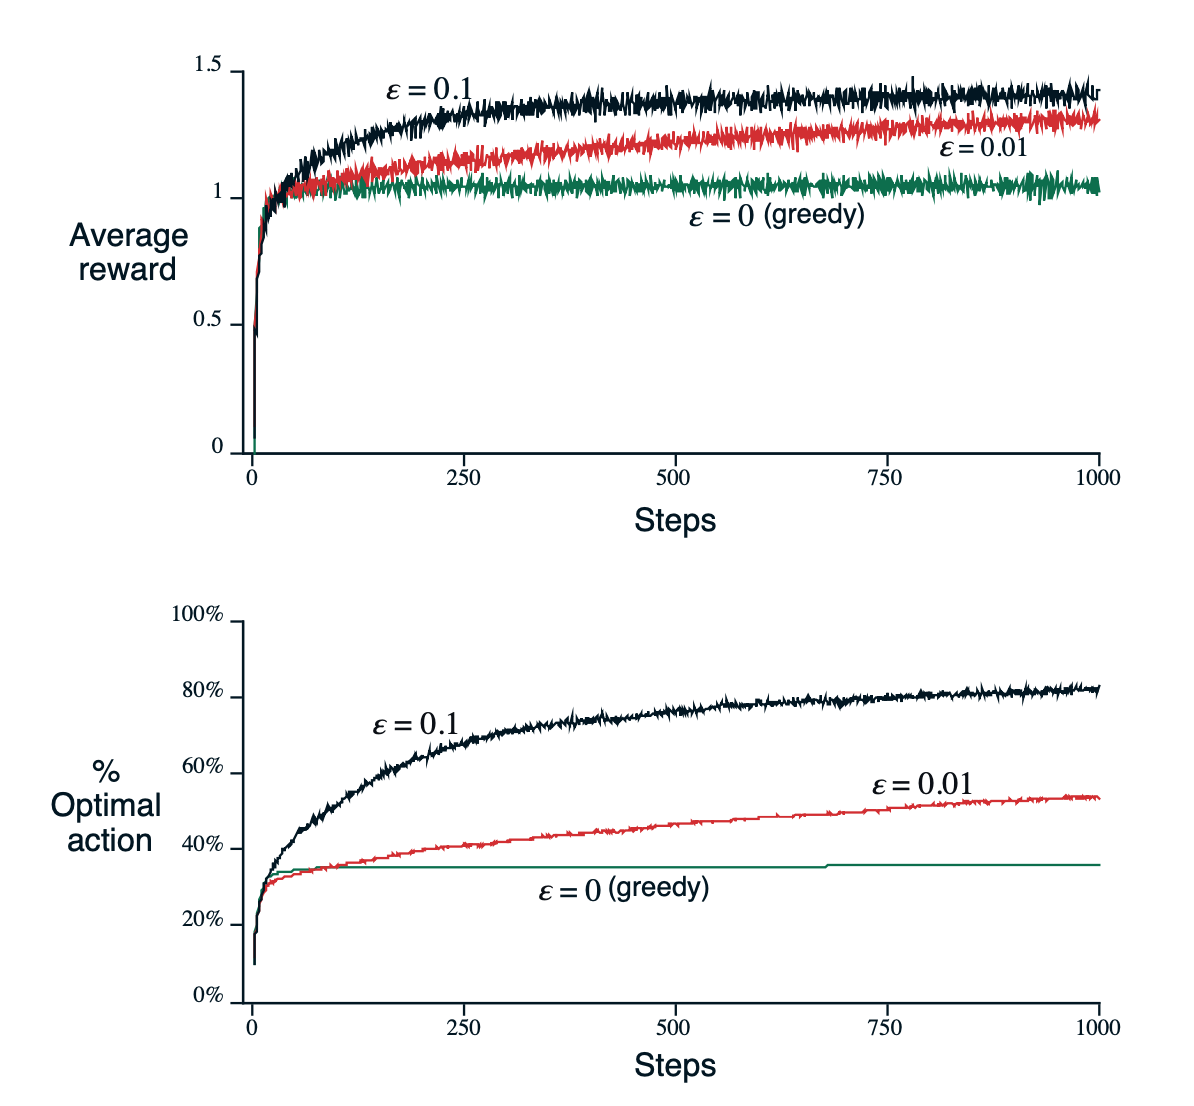
\includegraphics[width=0.8\textwidth]{/chapter2_1}
	\caption{Average performance of $\epsilon$-greedy action-value methods on the 10-armed testbed. These data are averages over 2000 runs with different bandit problems. All methods used sample averages as their action-value estimates.}
	\label{fig:chapter2_1}
\end{figure}

\subsection{Incremental Implementation}
The sample-average technique used to estimate action-values above has a problem: memory and computation requirements grow over time. This isn't necessary, we can devise an incremental solution instead:

\begin{align}
	Q_{k+1} &= \frac{1}{k}\sum_{i}^{k}R_i \nonumber \\
	&= \frac{1}{k} \left( R_k + \sum_{i=1}^{k-1} R_i \right) \nonumber \\
	&= \vdots \\
	&= Q_k + \frac{1}{k} \left[R_k - Q_k\right] \\
\end{align}

We are updating our estimate of \(Q_{k+1}\) by adding the discounted error between the reward just received and our estimate for that reward \(Q_k\).

\begin{equation}
NewEstimate \leftarrow OldEstimate + StepSize \left[Target - OldEstimate \right]
\end{equation}

\(\alpha\) is used to denote the stepsize (\(\frac{1}{k}\)) in the rest of this book.

\subsection{Tracking a Nonstationary Problem}
The averaging methods discussed above do not work if the bandit is changing over time. In such cases it makes sense to weight recent rewards higher than long-past ones. The popular way of doing this is by using a constant step-size parameter.

\begin{equation}
	Q_{k+1} = Q_k +\alpha \left[R_k - Q_k\right]
\end{equation}

where the step-size parameter \(\alpha \in (0,1]\) is constant. This results in \(Q_{k+1}\) being a weighted average of the past rewards and the initial estimate \(Q_1\):

\begin{align}
Q_{k+1} &= Q_k +\alpha \left[R_k - Q_k\right] \nonumber \\
&= \alpha R_k + (1 - \alpha)Q_k \nonumber \\
&= \alpha R_k + (1 - \alpha)[\alpha R_{k-1} + (1 - \alpha)Q_{k-1}] \nonumber \\
&= \alpha R_k + (1 - \alpha)\alpha R_{k-1} + (1 - \alpha)^2 Q_{k-1}  \nonumber \\
&= \vdots \nonumber \\
&= (1-\alpha)^k Q_1 + \sum_{i}^{k} \alpha (1 - \alpha)^{k-i} R_i \\
\end{align}

\begin{itemize}
\item Because the weight given to each reward depends on how many rewards ago it was observed, we can see that more recent rewards are given more weight. Note the weights \(\alpha\) sum to 1 here, ensuring it is indeed a weighted average where more weight is allocated to recent rewards.
\item In fact, the weight given to each reward decays exponentially into the past. This sometimes called an \textit{exponential} or \textit{recency-weighted} average.
\end{itemize}

\subsection{Optimistic Initial Values}
\begin{itemize}
\item The methods discussed so far are dependent to some extent on the initial action-value estimate i.e. they are biased by their initial estimates.
\item For methods with constant \(\alpha\) this bias is permanent.
\item In effect, the initial estimates become a set of parameters for the model that must be picked by the user.
\item In the above problem, by setting initial values to +5 rather than 0 we encourage exploration, even in the greedy case. The agent will almost always be disappointed with it's samples because they are less than the initial estimate and so will explore elsewhere until the values converge.
\item The above method of exploration is called \textit{Optimistic Initial Values}.
\end{itemize}

\subsection{Upper-confidence-bound Action Selection}
\(\epsilon\)-greedy action selection forces the agent to explore new actions, but it does so indiscriminately. It would be better to select among non-greedy actions according to their potential for actually being optimal, taking into account both how close their estimates are to being maximal and the uncertainty in those estimates. One way to do this is to select actions as:

\begin{equation}
	A_t = \argmax_a \left[Q_t(a) + c\sqrt{\frac{\ln t}{N_t(a)}}\right]
\end{equation}

where c \(>\) 0 controls the degree of exploration.

\begin{itemize}
	\item The square root term is a measure of the uncertainity in our estimate. It is proportional to \(t\) i.e. how many timesteps have passed and inversely proportional to \(N_t(a)\) i.e. how many times that action has been visited. The more time has passed, and the less we have sampled an action, the higher our upper-confidence-bound.
	\item As the timesteps increases, the denominator dominates the numerator as the ln term flattens.
	\item Each time we select an action our uncertainty decreases because N is the denominator of this equation.
	\item UCB will often perform better than e-greedy methods
\end{itemize}

\begin{figure}
	\centering
	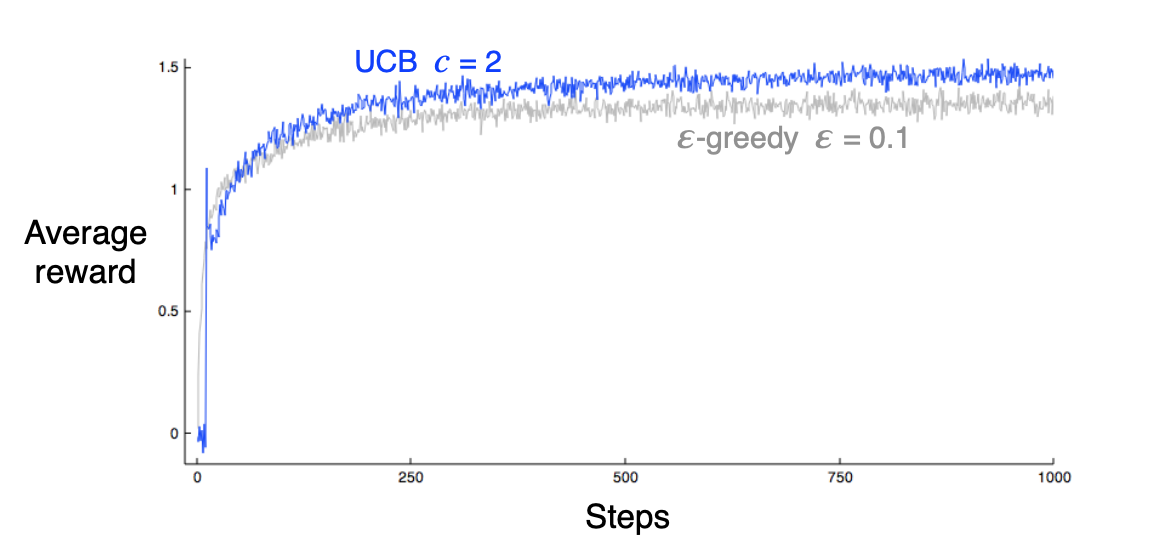
\includegraphics[width=0.8\textwidth]{/chapter2_2}
	\caption{UCB performs better than \(e\)-greedy in the n-armed bandit problem}
	\label{fig:chapter2_2}
\end{figure}

\subsection{Associative Search (Contextual Bandits)}
Thus far we have been discussing the stationary $k$-armed bandit problem, where the value of each arm is unknown but nonetheless remains stationary. Now, we consider a problem where the task could change from step to step, but the value distributions of the arms in each task remain the same. This is called contextual bandits, and in the toy example we are usually given a hint that the task has changed e.g. the slot machine changes colour for each task. Now we want to learn the correct action to take in a particular setting, given the task colour observed. This is an intermediary between the stationary problem and the full reinforcement learning problem. See exercise 2.10 below.

\subsection{Key Takeaways}
\begin{itemize}
\item The value of an action can be summarised by \(Q_t(a)\), the sample average return from an action
\item When selecting an action, it is preferable to maintain exploration, rather than only selecting the action we believe to be most valuable at any given timestep, to ensure we continue to improve our best estimate of the optimal action. We do so using \(\epsilon\))-greedy policies.
\item If our problem is non-stationary, rather than taking a standard average of every return received after an action, we can take a weighted average that gives higher value to more recently acquired rewards. We call this an \textit{exponential} or \textit{recency-weighted} average.
\item Optimistic initial values encourage lots of early exploration as our returns always decrease our estimate of \(Q_t\) meaning the greedy actions remain exploratory. Only useful for stationary problems.
\item \(\epsilon\)-greedy policies can be adapted to give more value to actions that have been selected less-often, i.e. actions where we have higher uncertainty in their value, using \textit{upper-confidence-bound} action selection.
\item Lastly, each of these techniques have varied performance on the n-armed bandit test dependent on their parametrisation. Their performance is plotted in Figure \ref{fig:chapter2_4}.
\end{itemize}

\begin{figure}
	\centering
	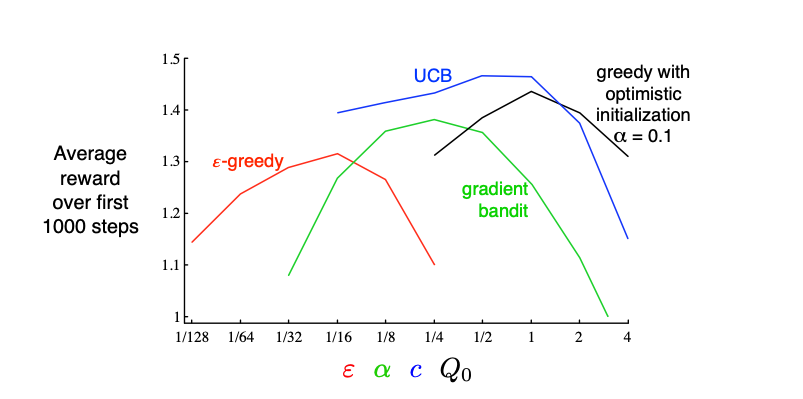
\includegraphics[width=0.8\textwidth]{/chapter2_4}
	\caption{Performance of each of the bandit algorithms explored in this chapter}
	\label{fig:chapter2_4}
\end{figure}


\section{Finite Markov Decision Processes}

\subsection{The Agent-Environment Interface}
\begin{figure}[h!]
	\centering
	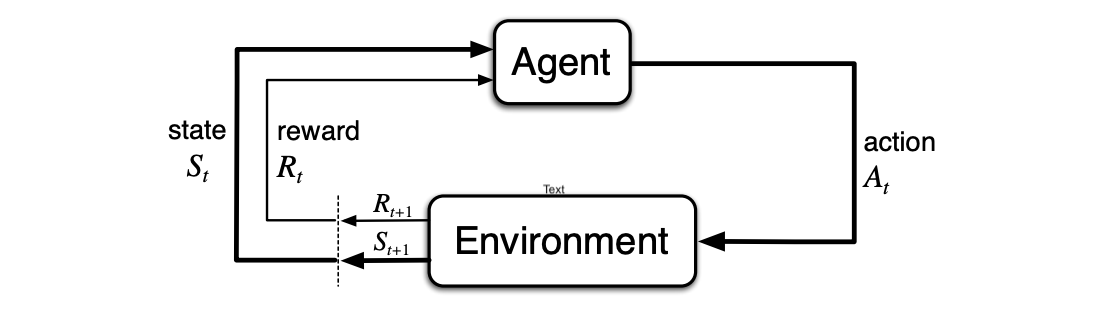
\includegraphics[width=\textwidth]{/chapter3_1}
	\caption{The agent-environment interface in reinforcement learning}
	\label{fig:agent-environment}
\end{figure}

\begin{itemize}
	\item At each timestep the agent implements a mapping from states to probabilities of selecting a possible action. The mapping is called the agents \textit{policy}, denoted \(\pi\), where \(\pi(a | s)\) is the probability of the agent selecting actions a in states.
	\item In general, actions can be any decision we want to learn how to make, and states can be any interpretation of the world that might inform those actions.
	\item The boundary between agent and environment is much closer to the agent than is first intuitive. E.g. if we are controlling a robot, the voltages or stresses in its structure are part of the environment, not the agent. Indeed reward signals are part of the environment, despite very possibly being produced by the agent e.g. dopamine.
\end{itemize}

\subsection{Goals and Rewards}
The \textit{reward hypothesis}:
\begin{displayquote}
	All we mean by goals and purposes can be well thought of as the maximization of the expected value of the cumulative sum of a received scalar signal (called reward).
\end{displayquote}

The reward signal is our way of communicating to the agent what we want to achieve not how we want to achieve it.

\subsection{Returns and Episodes}
The return \(G_t\) is the sum of future rewards:

\begin{equation}
	G_t = R_{t+1} + R_{t+2} + R_{t+3} + \cdots + R_t
\end{equation}

\begin{itemize}
	\item This approach makes sense in applications that finish, or are periodic. That is, the agent-environment interaction breaks into \textit{episodes}.
	\item We call these systems \textit{episodic tasks}. e.g playing a board game, trips through a maze etc.
	\item Notation for state space in an episodic task varies from the conventional case (\(s \in \mathcal{S}\)) to (\(s \in \mathcal{S^+}\))
	\item The opposite, continuous applications are called \textit{continuing tasks}.
	\item For these tasks we use \textit{discounted returns} to avoid a sum of returns going to infinity.
\end{itemize}

\begin{equation}
	G_t = R_{t+1} + \gamma R_{t+2} + \gamma^2 R_{t+3} + \cdots = \sum_{k=0}^{\infty} \gamma^k R_{t+k+1} 
\end{equation}

If the reward is a constant + 1 at each timestep, cumulative discounted reward $G_t$ becomes:

\begin{equation}
G_t = \sum_{k=0}^{\infty} \gamma^k = \frac{1}{1 - \gamma}
\end{equation}

\textit{Discounting} is a crucial topic in RL. It allows us to store a finite value of any state (summarised by its expected cumulative reward) for continuous tasks, where the non-discounted value would run to infinity. 

\subsection{Unified Notation for Episodic and Continuing Tasks}
\begin{equation}
	G_t = \sum_{k=0}^{T-t-1} \gamma^k R_{t+k+1} 
\end{equation}

\subsection{The Markov Property}
A state signal that succeeds in retaining all relevant information about the past is \textit{Markov}. Examples include:
\begin{itemize}
\item A cannonball with known position, velocity and acceleration
\item All positions of chess pieces on a chess board.
\end{itemize}

In normal causal processes, we would think that our expectation of the state and reward at the next timestep is a function of all previous states, rewards and actions, as follows:

\begin{equation}
	Pr \{R_{t+1} = r, S_{t+1} = s' | S_0, A_0, R_1, \ldots, S_{t-1}, A_{t-1}, R_t, S_t, A_t\}  
\end{equation}

If the state is Markov, however, then the state and reward right now completely characterizes the history, and the above can be reduced to:

\begin{equation}
p(s', r | s, a) = Pr \{R_{r+1} = r, S_{t+1} = s' | S_t, A_t\}
\end{equation}

\begin{itemize}
\item Even for non-Markov states, it is appropriate to think of all states as at least an approximation of a Markov state.
\item Markov property is important in RL because decisions and values are assumed to be a function only of the current state.
\item Most real scenarios are unlikely to be Markov. In the example of controlling HVAC, the HVAC motor might heat up which affects cooling power and we may not be tracking that temperature. It is hard for a process to be Markov without sensing all possible variables.
\end{itemize}

\subsection{Markov Decision Process (MDP)}
Given any state and action s and a, the probability of each possible pair of next state and reward, s', r is denoted:

\begin{equation}
p(s', r | s, a) = Pr \{R_{r+1} = r, S_{t+1} = s' | S_t, A_t\}
\end{equation}

We can think of \(p(s', r | s, a)\) as the dynamics of our MDP, often called the \textit{transition function}–it defines how we move from state to state given actions. 

\subsection{Policies and Value Functions}
\begin{itemize}
\item Value functions are functions of states or functions of state-value pairs.
\item They estimate how good it is to be in a given state, or how good it is to perform a given action in a given state.
\item Given future rewards are dependent on future actions, value functions are defined with respect to particular policies as the value of a state depends on the action an agent takes in said state.
\item A \textit{policy} is a mapping from states to probabilities of selecting each possible action.
\item RL methods specify how the agent's policy changes as a result of its experience.
\item For MDPs, we can define $v(\pi(s))$ formally as:
\end{itemize}

\begin{equation}
v_\pi(s) = \mathbb{E}_\pi \left[G_t | S_t = s \right] = \mathbb{E}_\pi \left[\sum_{k=0}^{\infty} \gamma^k R_{t+k+1} | S_t = s\right]
\end{equation}

i.e. the expected future rewards, given state \(S_t\), and policy \(\pi\). We call \(v_\pi(s)\)the \textit{state value function for policy} $\pi$. Similarly, we can define the value of taking action \(a\) in state \(s\) under policy \(\pi\) as:

\begin{equation}
q_\pi(s,a) = \mathbb{E}_\pi \left[G_t | S_t = s, A_t = a \right] = \mathbb{E}_\pi \left[\sum_{k=0}^{\infty} \gamma^k R_{t+k+1} | S_t = s, A_t = a \right]
\end{equation}

i.e. the expected value, taking action \(a\) in state \(s\) then following policy \(\pi\).
\begin{itemize}
\item We call \(q_\pi\) the \textit{action-value function for policy \(\pi\)}
\item Both value functions are estimated from experience.
\end{itemize}

A fundamental property of value functions used throughout reinforcement learning and dynamic programming is that they satisfy recursive relationships similar to that which we have already established for the return. This recursive relationship is characterised by the \textit{Bellman Equation}:

\begin{equation}
v_\pi(s) = \sum_{a} \pi(a|s) \sum_{s',r} p(s', r | s, a) \left[r + \gamma v_\pi(s')\right]
\end{equation}

This recursion looks from one state through to all possible next states given our policy and the dynamics as suggested by \ref{fig:backup}:
\begin{figure}[h!]
	\centering
	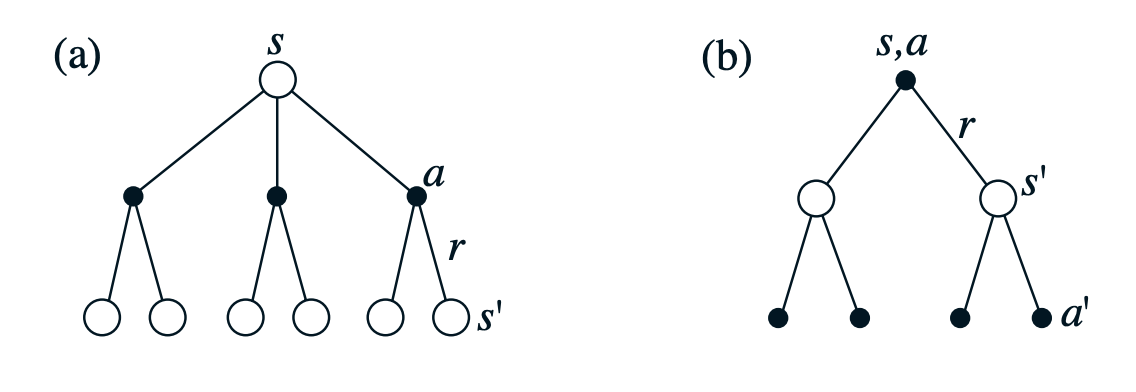
\includegraphics[width=\textwidth]{/chapter3_2}
	\caption{Backup diagrams for \(v_\pi\) and \(q_\pi\)}
	\label{fig:backup}
\end{figure}

\subsection{Optimal Policies and Value Functions}
\begin{itemize}
\item A policy \(\pi '\) is defined as better than policy pi if its expected return is higher for all states.
\item There is always \textit{at least} one policy that is better than or equal to all other policies - this is the \textit{optimal policy}.
\item Optimal policies are denoted \(\pi_*\)
\item Optimal state-value functions are denoted \(v_*\)
\item Optimal action-value functions are denoted \(q_*\)
\item We can write \(q_*\) in terms of \(v_*\):
\end{itemize}

\begin{equation}
q_*(s,a) = \mathbb{E} \left[R_{t+1} + \gamma v_*(S_{t+1}) | S_t = s, A_t = a \right]
\end{equation}

We can adapt the Bellman equation to achieve the Bellman optimality equation, which takes two forms. Firstly for \(v_*\):
\begin{equation}
v_*(s) = \max_{a \in \mathcal{A}(s)} \sum_{s',r} p(s', r | s, a) \left[r + \gamma v_*(s')\right]
\end{equation}
and secondly for \(q_*\):
\begin{equation}
q_*(s) = \sum_{s',r} p(s', r | s, a) \left[r + \gamma \max_{a'} q_*(s', a') \right]
\end{equation}

\begin{itemize}
\item Using \(v_*\) the optimal expected long term return is turned into a quantity that is immediately available for each state. Hence a one-step-ahead search, acting greedily, yield the optimal long-term actions.
\item Fully solving the Bellman optimality equations can be hugely expensive, especially if the number of states is huge, as is the case with most interesting problems.
\item Solving the Bellman optimality equation is akin to exhaustive search. We play out \textit{every} possible scenario until the terminal state and collect their expected reward. Our policy then defines the action that maximises this expected reward. 
\item In the continuous case the Bellman optimality equation is unsolvable as the recursion on the next state's value function would never end.
\end{itemize}

\subsection{Optimality and Approximation}
\begin{itemize}
	\item We must approximate because calculation of optimality is too expensive.
	\item A nice way of doing this is allowing the agent to make sub-optimal decisions in scenarios it has low probability of encountering. This is a trade off for being optimal in situations that occur frequently.
\end{itemize}

\subsection{Key Takeaways}
\begin{itemize}
\item We summarise our goal for the agent as a \textit{reward}; its objective is to maximise the cumulative sum of future rewards
\item For episodic tasks, returns terminate (and are backpropogated) when the episode ends. For the continuous control case, returns are discounted so they do not run to infinity. 
\item A state signal that succeeds in retaining all relevant information about the past is \textit{Markov}. 
\item Markov Decision Processes (MDPs) are the mathematically idealised version of the RL problem. They have system dynamics: $p(s', r | s, a) = Pr \{R_{r+1} = r, S_{t+1} = s' | S_t, A_t\}$
\item Policies are a (probabilistic) mapping from states to actions.
\item Value functions estimate how good it is for an agent to be in a state ($v_\pi$) or to take an action from a state ($q_\pi$). They are always defined w.r.t policies as the value of a state depends on the policy one takes in that state. Value functions are the \textit{expected cumulative sum of future rewards} from a state or state-action pair.
\item Knowing our policy and system dynamics, we can define the state value function is defined by the Bellman equation: $v_\pi(s) = \sum_{a} \pi(a|s) \sum_{s',r} p(s', r | s, a) \left[r + \gamma v_\pi(s')\right]$
\item An optimal policy ($\pi_*$) is the policy that maximises expected cumulative reward from all states. From the optimal policy we can derive the optimal value functions $q_*$ and $v_*$.
\end{itemize}











\section{Dynamic Programming}

\subsection{Policy Evaluation}
\begin{itemize}
\item Computing the value function for an arbitrary policy \(\pi\). Ideally, we would do this using dynamic programming if the state-space is finite and we know the state transition perfectly.
\end{itemize}


\subsection{Policy Improvement}
\begin{itemize}
\item Take our policy and associated value function obtained through policy evaluation. Then in state s, we take a different action `a` not prescribed by our policy, follow our normal policy thereafter, and see if the value function changes. If the value of that state improves then we say that our policy has improved.
\item If we extend this to the limit and choose to take the value-maximising action in each state we call this acting greedily with respect to our value function.
\end{itemize}


\subsection{Policy Iteration}
By flipping between policy evaluation and iteration we can achieve a sequence of monotonically increasing policies and value functions. Algorithm is:
\begin{enumerate}
\item Evaluate policy \(\pi\) to obtain value function \(V_\pi\)
\item Improve policy \(\pi\) by acting greedily with respect to \(V_\pi\) to obtain new policy \(\pi'\)
\item Evaluate new policy \(\pi'\) to obtain new value function `\(V_{\pi'}\)
\item Repeat until new policy is no longer better than the old policy, at which point we have obtained the optimal policy. (Only for finite MDPs)
\end{enumerate}

\subsection{Key Takeaways}

\section{Monte Carlo Methods}
If we do not have knowledge of the transition probabilities (model of the environment) then we must learn directly from experience. To do so, we use Monte Carlo methods. Monte carlo methods are most effective in episodic tasks where there is a terminal state and the value of the states visited en route to the terminal state can be updated based on the reward received at the terminal state. We use general policy iteration as outlined in chapter 4, but this time instead of \textit{computing} the value function we learn it from samples. We first consider the prediction problem to obtain $v_\pi$ and/or \textbf{$q_\pi$} for a fixed policy, then we look to improve using policy improvement, then we use it for control.  

\subsection{Monte Carlo Policy Prediction}
\begin{itemize}
\item Recall that the value of a state is the expected discounted future reward from that state. One way of estimating that value is by observing the rewards obtained after visiting the state, we would expect that in the limit this would converge toward the true value.
\item We can therefore run a policy in an environment for an episode. When the episode ends, we receive a reward and we assign that reward to each of the states visited en route to the terminal state. 
\item Where DP algorithms perform one-step predictions to \textit{every} possible next state; monte-carlo methods only sample one trajectory/episode. This can be summarised in a new backup diagram as follows:
\begin{figure}[h!]
	\centering
	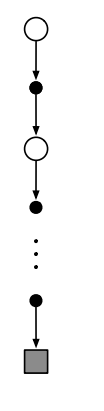
\includegraphics[width=0.1\textwidth]{/chapter5_1}
	\caption{Monte carlo backup diagram for one episode}
	\label{fig:monte carlo backup}
\end{figure}

\item Importantly, monte carlo methods do not bootstrap in the same way DP methods do. They take the reward at the end of an episode, rather than estimated reward based on the value of the next state.
\item Because of the lack of bootstrapping, this expense of estimating the value of one state is independent of the number of states, unlike DP. A significant advantage, in addition to the other advantages of being able to learn from experience without a model or from simulated experience. 
\end{itemize}

\subsection{Monte Carlo Estimation of Action Values}
\begin{itemize}
\item With a model we only need to estimate the state value function \(v\) as, paired with our model, we can evaluate the rewards and next states for each of our actions and pick the best one.
\item With model free methods we need to estimate the state-action value function \(q\) as we must explicitly estimate the value of each action in order for the values to be useful in suggesting a policy. (If we only have the values of states, and don't know how states are linked through a model, then selecting the optimal action is impossible)
\item One serious complication arises when we do not visit every state, as can be the case if our policy is deterministic. If we do not visit states then we do not observe returns from these states and cannot estimate their value. We therefore need to \textit{maintain exploration} of the state space. One way of doing so is stochastically selected a state-action pair to start an episode, giving every state-action pair a non-zero probability of being selected. In this case, we are said to be utilising \textit{\textbf{exploring starts}}.
\item Exploring starts falls down when learning from real experience because we cannot guarantee that we start in a new state-action pair in the real world. 
\item An alternative approach is to use stochastic policies that have non-zero probability of selecting each state-action pair.
\end{itemize}


\subsection{Monte Carlo Control}
\begin{itemize}
\item Much like we did with value iteration, we do not need to fully evaluate the value function for a given policy in monte carlo control. Instead we can merely \textit{move} the value toward the correct value and then switch to policy improvement thereafter. It is natural to do this episodically i.e. evaluate the policy using one episode of experience, then act greedily w.r.t the previous value function to improve the policy in the next episode.
\item If we use a deterministic policy for control, we must use exploring starts to ensure sufficient exploration. This creates the \textit{Monte Carlo ES} algorithm.
\end{itemize}

\subsection{Monte Carlo Control without Exploring Starts}
\begin{itemize}
\item To avoid having to use exploring starts we can use either \textit{on-policy} or \textit{off-policy} methods. The only way to ensure we visit everything is to visit them directly.
\item On-policy methods attempt to improve or evaluate or improve the policy that is making decisions.
\item On-policy control methods are generally \textit{soft} meaning that they assign non-zero probability to each possible action in a state e.g. e-greedy policies.
\item We take actions in the environment using e-greedy policy, after each episode we back propagate the rewards to obtain the value function for our e-greedy policy. Then we perform policy improvement by updating our policy to take the \textbf{new} greedy reward in each state. Note: based on our new value function, the new greedy action may have changed in some states. Then we perform policy evaluation using our new e-greedy policy and repeat (as per generalised policy iteration).
\item The idea of on-policy Monte Carlo control is still that of GPI. We use first visit MC methods to estimate the action-value function i.e. to do policy evaluation, but we cannot then make improve our policy merely by acting greedily w.r.t our value function because that would prevent further exploration of non-greedy actions. We must maintain exploration and so improve the $\epsilon$-greedy version of our policy. That is to say, when we find the greedy action (the action that maximises our reward for our given value function) we assign it probability $1 - \epsilon + \frac{\epsilon}{\mathcal{A}(S_t)}$ of being selected so that the policy remains stochastic.
\item Note: doing the above will only find us the best policy amongst the $\epsilon$-soft policies, which may not be the optimal policy for the environment, but it does allow us to remove the need for exploratory starts.
\end{itemize}

\subsection{Off-policy Prediction via Importance Sampling}
We face a dilemma when learning control: we want to find the optimal policy, but we can only find the optimal policy by acting suboptimally to explore sufficient actions. What we saw with on-policy learning was a compromise - it learns action values not for the optimal policy but for a near-optimal policy that still explores. An alternative is off-policy control where we have two policies: one used to generate the data (behaviour policy) and one that is learned for control (target policy). This is called \textit{off policy learning}.

\begin{itemize}
\item Off-policy learning methods are powerful and more general than on-policy methods (on-policy methods being a special case of off-policy where target and behaviour policies are the same). They can be used to learn from data generated by a conventional non-learning controller or from a human expert.
\item If we consider an example of finding target policy $\pi$ using episodes collected through a behaviour policy $b$, we require that every action in $\pi$ must also be taken, at least occasionally, by $b$ i.e. $\pi(a|s) > 0$ implies $b(a|s) > 0$. This is called the assumption of \textit{\textbf{coverage}}. 
\item Almost all off-policy methods utilize \textit{importance sampling}, a general technique for estimating expected values under one distribution given samples from another. Given a starting state $S_t$, the probability of the subsequent state-action trajectory occuring under any policy $\pi$ is:

\begin{equation}
	\prod_{k=t}^{T-1} \pi(A_k|S_k)p(S_{k+1}|S_k, A_k)
\end{equation}

where $p$ is the state transition probability function. We can then obtain the relative probability of the trajectory under the target and behaviour policies (the importance sampling ratio) as:

\begin{equation}
p_{t:T-1} = \frac{\prod_{k=t}^{T-1} \pi(A_k|S_k)p(S_{k+1}|S_k, A_k)}{\prod_{k=t}^{T-1} b(A_k|S_k)p(S_{k+1}|S_k, A_k)} = \prod_{k=t}^{T-1} \frac{\pi(A_k|S_k)}{b(A_k|S_k)}
\end{equation}

We see here that the state transition probability function helpfully cancels.

\item We want to estimate the expected returns under the target policy but we only have returns from the behaviour policy. To address this we simply multiply expected returns from the behaviour policy by the importance sampling ratio to get the value function for our target policy.

\begin{equation}
\mathbb{E} \left[p_{t:T-1} G_t | S_t = s\right] = v_\pi(s)
\end{equation}

\item Note: importance sampling ratios are only non-zero for episodes where the target-policy has non-zero probability of acting \textit{exactly} like the behaviour policy $b$. So, if the behaviour policy takes 10 steps in an episode, each of these 10 steps have to have been \textit{possible} by the target policy, else $\pi(a|s) = 0$ and $\rho_{t:T-1} = 0$.

\end{itemize}

\subsection{Incremental Implementation}
We perform monte carlo policy evaluation (prediction) incrementally in the same way as was done in Chapter 2 for the bandit problem. Generally incremental implementation follows this formula:

\begin{equation}
New Estimate \leftarrow Old Estimate + Step Size \left[Observation - Old Estimate \right]
\end{equation}

With on-policy monte carlo methods, this update is performed exactly after each episode for each visit to a state given the observed rewards, with off-policy methods the update is slightly more complex. With ordinary importance sampling, the step size is $1/n$ where $n$ is the number of visits to that state, and so acts as an average of the scaled returns. For weighted importance sampling, we have to form a weighted average of the returns which requires us to keep track of the weights. If the weight takes the form $W_i = \rho_{t:T(t)-1}$ then our update rule is:

\begin{equation} \label{incremental V}
V_{n+1} = V_n + \frac{W_n}{C_n}\left[G_n - V_n\right]
\end{equation}
where,
\begin{equation}
C_{n+1} = C_n + W_{n+1}
\end{equation}
with $C_0 = 0$. This allows us to keep tracking of the corrected weighted average term for each update as they are made. Note here that the weighted average gives more weight to updates based on common trajectories from $b$ in $\pi$ that we have some more often.

\subsection{Off-policy Monte Carlo Control}
Using incremental implementation (updates to the value function) and importance sampling we can now discuss \textit{off-policy monte carlo control}–the algorithm for obtaining optimal policy $\pi_*$ by using rewards obtained through behaviour policy $b$. This works in much the same way as in previous sections; $b$ must be $\epsilon$-soft to ensure the entire state space is explored in the limit; updates are only made to our estimate for $q_\pi$, $Q$, if the sequence of states an actions produced by $b$ could have been produced by $\pi$. This algorithm is also based on GPI: we update our estimate of $Q$ using Equation \ref*{incremental V}, then update $\pi$ by acting greedily w.r.t to our value function. If this policy improvement changes our policy such that the trajectory we are in from $b$ no longer obeys our policy, then we exit the episode and start again. The full algorithm is shown in \ref*{fig:Off-policy monte carlo control}.

\begin{figure}[h!]
	\centering
	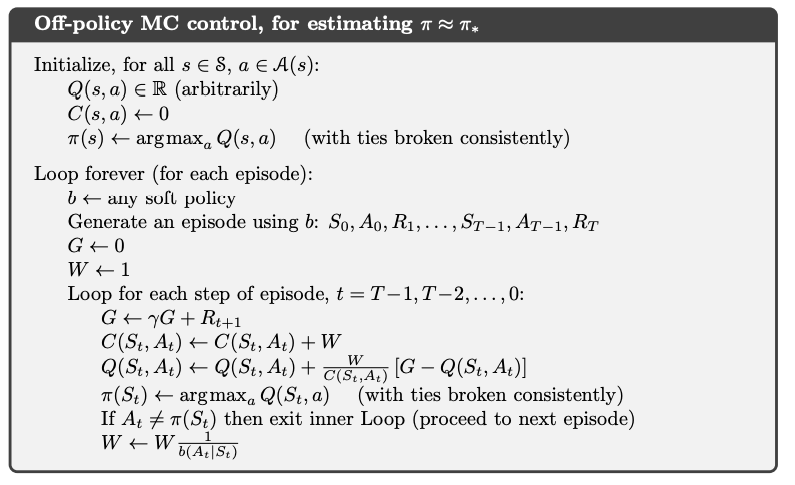
\includegraphics[width=0.5\textwidth]{/chapter5_3}
	\caption{Off-policy monte carlo control}
	\label{fig:Off-policy monte carlo control}
\end{figure}

\subsection{Key Takeaways}
\begin{itemize}
\item In the absence of a model of the environment, monte carlo methods allow us to evaluate and improve our value function based on \textit{experience}
\item We roll-out trajectories to terminal states, and back-propagate the rewards to the states visited en-route in several ways
\item Monte carlo methods use GPI (see chapter 4) in much the same way dynamic programming does. We evaluate our policy, then improve by acting greedily w.r.t our new value function until we converge on the optimal value function and policy.
\item Differences with dynamic programming methods: 1) They do not require a model of the environment as they learn directly from experience, and 2) They do not bootstrap i.e. the value function estimates are an average of all real returns accumulated after visiting the state.
\item Maintaining sufficient exploration is crucial with monte carlo methods; if our policy is deterministic we will likely not explore the full states space during our roll-outs. To deal with this we have several options: 1) Start every episode randomly with uniform probability such that we make sure we start at each possible state–called \textit{exploring starts}, unrealistic in the real world as we can't make a robot restart from all possible states. Or 2) Use $\epsilon$-soft policies that have a non-zero probability of selecting all possible states. The downside of doing this is that we will converge on the optimal $\epsilon$-soft, which is not necessarily the optimal policy for the environment, because it needs to learn how account for its own randomness. This is the price we pay for exploration.
\item Monte carlo methods can either be \textit{on-policy} or \textit{off-policy}.
\item On-policy methods use the same policy to collect data as is evaluated and improved. This suffers the downsides outlined above.
\item Off-policy methods have two policies, one that collects the data called the \textit{behaviour policy} $b$ and the other which we look to improve called the target policy $\pi$. We find trajectories from the behaviour policy that line up with our target policy, that is to say, that could have been produced by our target policy. This process only works if the behaviour policy has non-zero probability of selecting each of the actions in the target policy, aka \textit{coverage} of the target policy. The agent explores, but learns a deterministic optimal policy offline that may be unrelated to the behaviour policy used to collect the experience.
\item Based on rewards observed by running the behaviour policy, we update our value function using \textit{importance sampling}, which measures, if effect, how likely the observed behaviour would have been given our target policy. For example, the target policy may take 1 of 4 actions with equal probability in each state. If we observe two timesteps from our beaviour policy, then our probability of selecting the actions taken by the behaviour policy would be $0.25 x 0.25$. 
\item We weight each return using the x\textit{importance sampling ratio}, a measure of how likely we were to produce the roll-out using the target policy compared to how likely we were to produce the roll-out using the behaviour policy. 
\item Importance sampling can be \textit{ordinary} i.e. an average of the returns observed from a state or \textit{weighted} where trajectories viewed more often, or with a higher importance sampling ratio give the value update more weight.

\end{itemize}

\end{document}